\section{Methodology}
\label{sec:methodology}

DynSTEER establishes an end-to-end framework for dynamic agent trajectory evaluation, as illustrated in Figure~\ref{fig:overall_framework}. Rather than treating rollouts as opaque black boxes or enforcing rigid single-path matching, DynSTEER coordinates three core components: pre-execution milestone graph generation to preserve execution diversity (Section~\ref{sec:blueprint_compilation}); stage-wise trajectory evaluation anchored by action closures and dominators (Section~\ref{sec:stage_alignment}); and dynamic strategy adaptation with execution-time early termination to focus on weak segments and curb resource waste (Section~\ref{sec:routing_early_stop}).

\begin{figure*}[t]
\centering
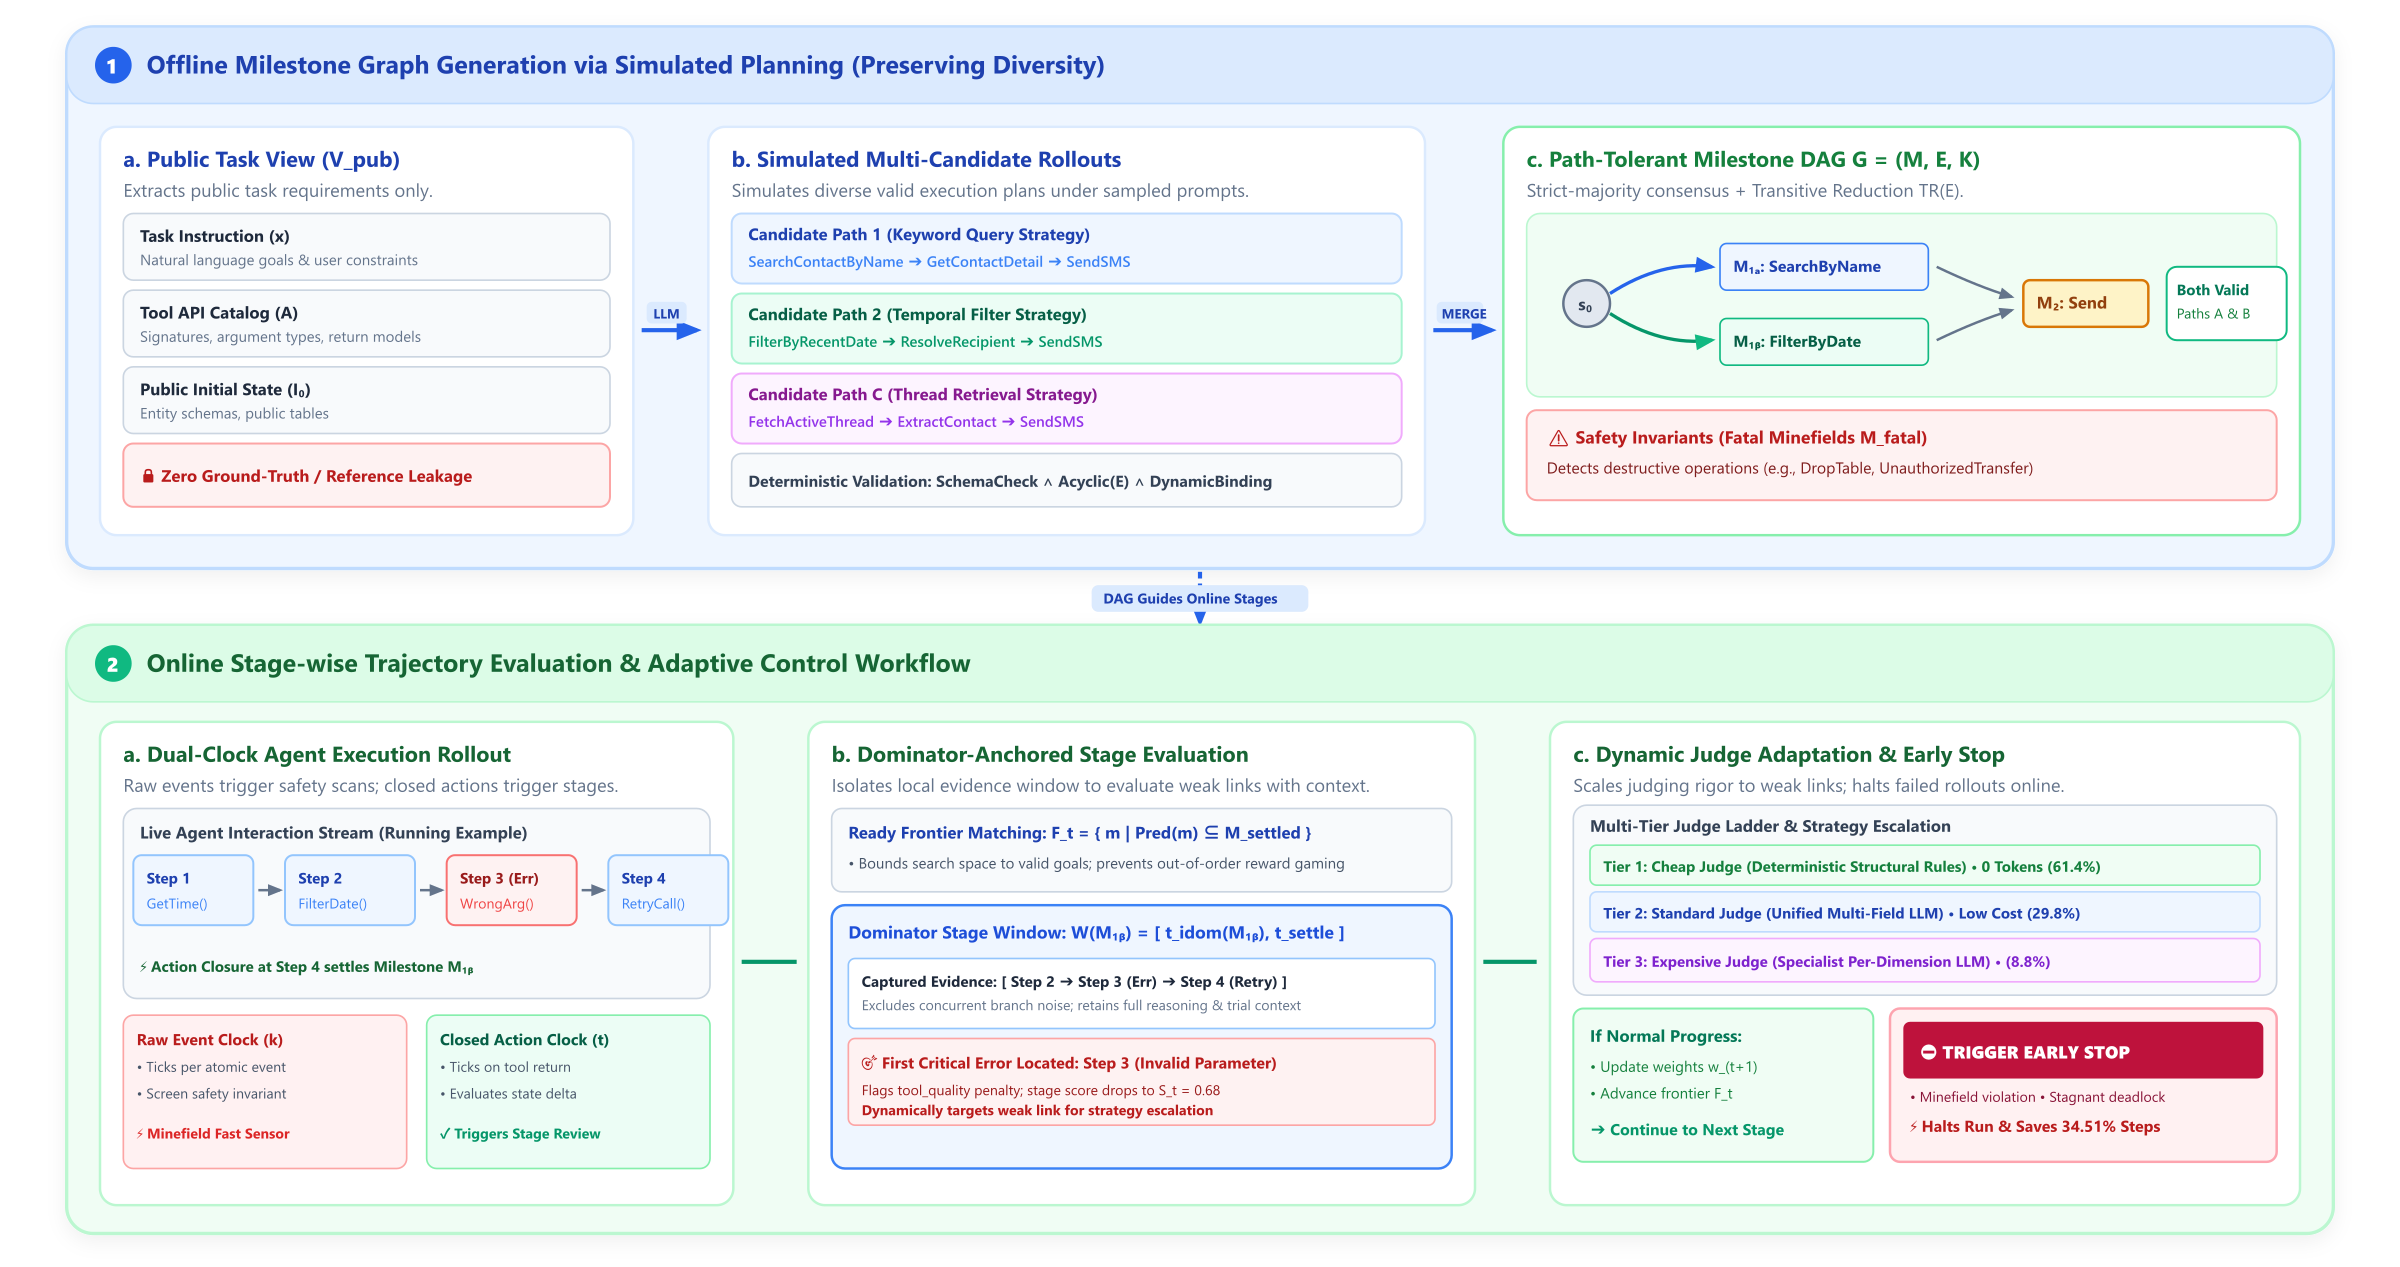
\includegraphics[width=0.96\textwidth]{figures/overall-framework.png}
\vspace{-0.25cm}
\caption{\textbf{Overview of the \textsc{DynSTEER} Workflow.} (1) Pre-execution milestone graph generation synthesizes multi-candidate simulated rollouts from public views to compile a path-tolerant DAG. (2) Online stage-wise evaluation aligns closed actions, isolates dominator evidence windows to evaluate weak links with trajectory context, adaptively scales judge tiers, and halts unrecoverable executions online.}
\label{fig:overall_framework}
\vspace{-0.35cm}
\end{figure*}

\subsection{Problem Formulation and Dual-Clock Observation Model}
\label{sec:formulation}
Following standard formulations of interactive tool-using agent environments~\citep{gu2024toolsandbox,yang2023intercode,liu2023agentbench}, an agent task is formalized as a tuple $T = (x, \mathcal{S}_0, \mathcal{A}, \mathcal{C})$, where $x$ represents the user instruction, $\mathcal{S}_0$ is the initial environment state, $\mathcal{A}$ denotes the catalog of accessible tool APIs with input/output parameter schemas, and $\mathcal{C}$ defines environment state invariants and safety contracts. To preserve evaluation integrity and prevent test contamination, DynSTEER operates strictly over the \textbf{public task view}:
\begin{equation}
    V_{\text{public}} = (x, \mathcal{A}, \mathcal{I}_0)
    \label{eq:v_public}
\end{equation}
where $\mathcal{I}_0$ denotes public metadata (e.g., initial database entity headers), strictly isolating any hidden reference paths $\tau^*$ or terminal unit tests.

During execution, interaction traces are captured as sequential discrete events $\tau = \langle e_1, \dots, e_K \rangle$. To balance continuous safety screening with accurate semantic evaluation, DynSTEER introduces a \textbf{dual-clock observation model}:
\begin{itemize}[leftmargin=*,itemsep=1.5pt,topsep=1pt]
    \item \textbf{Raw Event Clock ($k \in \{1, \dots, K\}$):} Increments at every atomic event, including thoughts, tool calls, and environment responses, dedicated to instant safety interception of fatal minefield operations $e_k \in \mathcal{M}_{\text{fatal}}$.
    \item \textbf{Closed Action Clock ($t \in \{1, \dots, T\}$):} Advances only when an action reaches semantic closure---specifically, when a tool call receives its execution return, and the agent yields control. Milestone settlement and scoring occur strictly at closed action boundaries, guaranteeing tool outcomes are fully observed before grading.
\end{itemize}

\subsection{Milestone Graph Generation via Simulated Planning}
\label{sec:blueprint_compilation}
To overcome single-reference bias, DynSTEER compiles $V_{\text{public}}$ into a path-tolerant Milestone DAG $G = (M, E, \mathcal{K}, \mathcal{M}_{\text{fatal}})$ prior to execution, where $M$ is the milestone set, $E$ encodes precedence constraints, $\mathcal{K}$ specifies parameter bindings, and $\mathcal{M}_{\text{fatal}}$ defines hazardous operations.

\textbf{Multi-Candidate Synthesis and Contract Validation.} Given $V_{\text{public}}$, a blueprint generator synthesizes $C$ candidate plans $\{G_1, \dots, G_C\}$ via temperature-sampled LLM prompting across diverse exploration heuristics (e.g., direct keyword queries vs. hierarchical filtering). Each candidate $G_c = (M_c, E_c)$ undergoes deterministic contract verification:
\begin{equation}
    \text{Valid}(G_c) = \text{SchemaCheck}(M_c, \mathcal{A}) \land \text{Acyclic}(E_c) \land \text{BindingConsistency}(\mathcal{K}_c)
    \label{eq:valid_gc}
\end{equation}
Pruning candidates with hallucinated APIs, type mismatches, or cyclic dependencies.

\textbf{Strict-Majority Consensus and Transitive Reduction.} To retain essential invariants while preserving exploratory flexibility, a milestone $m$ is retained if and only if it appears in a strict majority of valid candidates:
\begin{equation}
    M = \left\{ m \;\middle|\; \sum_{c=1}^{C_{\text{valid}}} \mathbb{I}[m \in M_c] \ge \left\lceil \frac{C_{\text{valid}} + 1}{2} \right\rceil \right\}
    \label{eq:consensus}
\end{equation}
Precedence edges are aggregated analogously. Finally, we compute the transitive reduction $E = \text{TR}(E_{\text{majority}})$~\citep{tarjan1972depth} to eliminate redundant shortcut dependencies, producing a minimal DAG that accommodates diverse legitimate execution strategies.

\subsection{Stage-wise Trajectory Evaluation}
\label{sec:stage_alignment}
During execution, DynSTEER dynamically aligns closed actions against the milestone DAG (complete algorithmic flow in Algorithm~\ref{alg:dynsteer} in Appendix~\ref{app:algorithms}).

\textbf{Ready Frontier Matching.} Let $M_{<t}$ denote milestones settled prior to closed action $t$. The active search space is strictly bounded by the \textbf{ready frontier}:
\begin{equation}
    \mathcal{F}_t = \{ m \in M \setminus M_{<t} \mid \text{Pred}(m) \subseteq M_{<t} \}
    \label{eq:frontier}
\end{equation}
An action $a_t$ settles milestone $m^* \in \mathcal{F}_t$ if its tool call and state delta satisfy semantic predicates $\phi_{m^*}(a_t, s_t) = 1$. Restricting alignment to $\mathcal{F}_t$ prevents out-of-order settlement and reward gaming.

\textbf{Dominator-Anchored Stage Isolation.} To evaluate $m^*$ without contamination from concurrent parallel branches, DynSTEER computes the immediate dominator $\text{idom}(m^*)$ in $G$~\citep{lengauer1979fast}, defined as the unique node that must be traversed on every directed path from start node $s_0$ to $m^*$. The \textbf{stage evidence window} is bounded by:
\begin{equation}
    \mathcal{W}(m^*) = [t_{\text{idom}(m^*)}, t]
    \label{eq:stage_window}
\end{equation}
where $t_{\text{idom}(m^*)}$ is the execution step at which the dominator was settled. Isolating evidence to $\mathcal{W}(m^*)$ excludes unrelated actions from parallel branches while capturing all intermediate reasoning, trial-and-error attempts, and parameter adjustments leading directly to $m^*$. Unlike whole-trajectory evaluation, which obscures mistake locations, and single-step evaluation, which lacks context, dominator-anchored stages provide enough trajectory context to evaluate intermediate quality and pinpoint the exact first-error step.

\textbf{Multidimensional Quality Scoring.} Once settled, milestone $m^*$ is scored across four orthogonal dimensions: Correctness ($c$), Efficiency ($\eta$), Safety ($s$), and Tool Compliance ($\kappa$). The composite stage score is:
\begin{equation}
    S_t = \sum_{d \in \mathcal{D}} w_d^{(t)} s_d^{(t)}(m^*)
    \label{eq:stage_scoring}
\end{equation}
parameterized by dynamically normalized weights $\mathbf{w}^{(t)}$.

\subsection{Dynamic Judge Adaptation and Early Termination}
\label{sec:routing_early_stop}
A central innovation of DynSTEER is dynamically adapting evaluation strategies to an agent's intermediate vulnerabilities and halting unpromising rollouts during execution.

\textbf{Multi-Tier Judge Structure.} Rather than assigning a uniform evaluator across all stages, DynSTEER deploys a three-tier judge hierarchy (prompt templates in Appendix~\ref{app:prompts}):
\begin{itemize}[leftmargin=*,itemsep=1.5pt,topsep=1pt]
    \item \textbf{Tier 1: Cheap Judge ($J_{\text{cheap}}$):} A deterministic structural evaluator inspecting tool status codes, schemas, and evidence rules without LLMs, incurring zero model inference overhead.
    \item \textbf{Tier 2: Standard Judge ($J_{\text{std}}$):} A multi-field unified LLM evaluator scoring all target dimensions simultaneously within a single structured JSON pass, aggregating confidence across multiple samples.
    \item \textbf{Tier 3: Expensive Judge ($J_{\text{exp}}$):} A single-dimension specialist LLM evaluator executing dedicated expert rubrics and deep counterfactual analysis across multiple deliberation passes to capture subtle behavioral defects.
\end{itemize}

\textbf{Dynamic Strategy Adjustment.} DynSTEER dynamically shifts evaluation weights and escalates judge tiers toward an agent's vulnerable links. First, dimension weights are updated via exponential gradient scaling:
\begin{equation}
    w_d^{(t+1)} = \frac{w_d^{(t)} \cdot \exp\left( \alpha (1 - s_d^{(t)}) + \beta u_d^{(t)} \right)}{\sum_{d' \in \mathcal{D}} w_{d'}^{(t)} \cdot \exp\left( \alpha (1 - s_{d'}^{(t)}) + \beta u_{d'}^{(t)} \right)}
    \label{eq:weight_update}
\end{equation}
where $s_d^{(t)} \in [0, 1]$ is the dimension score, $u_d^{(t)} \in [0, 1]$ is dimension uncertainty, and $\alpha, \beta$ scale sensitivity to quality deficits and uncertainty. Second, the baseline judge tier is set to:
\begin{equation}
    \text{Level}_{\text{base}}^{(t+1)} = 
    \begin{cases}
    J_{\text{cheap}}, & \text{if } S_t \ge \theta_{\text{pass}} + \delta_{\text{margin}} \;\land\; \max_{d} u_d^{(t)} \le \theta_{\text{low\_u}} \;\land\; \mathcal{M}_{\text{fatal}}^{(t)} = 0 \\
    J_{\text{std}}, & \text{otherwise}
    \end{cases}
    \label{eq:level_base}
\end{equation}
For each individual dimension $d$, its tier $\text{Level}_d^{(t+1)}$ adaptively escalates along $J_{\text{cheap}} < J_{\text{std}} < J_{\text{exp}}$:
\begin{equation}
    \text{Level}_d^{(t+1)} = 
    \begin{cases}
    J_{\text{exp}}, & \text{if } s_d^{(t)} < \theta_{\text{fail}} \\
    \min\left(J_{\text{exp}},\, \text{Level}_d^{(t)} + 1\right), & \text{if } s_d^{(t)} < \theta_{\text{warn}} \lor u_d^{(t)} \ge \theta_{\text{high\_u}} \\
    \text{Level}_{\text{base}}^{(t+1)}, & \text{otherwise}
    \end{cases}
    \label{eq:level_dim}
\end{equation}
This focuses expensive LLM deliberation selectively on weak or ambiguous execution links while relaxing confident stages to rule-based verification in $J_{\text{cheap}}$ to minimize unnecessary LLM invocations.

\textbf{Execution-Time Early Termination.} To prevent runaway executions on unrecoverable trajectories, DynSTEER monitors four stopping criteria: (1) \textbf{Fatal Minefield Interception ($e_k \in \mathcal{M}_{\text{fatal}}$)}, halting immediately on the raw event clock upon hazardous or irreversible actions; (2) \textbf{Structural Invariant Failures}, catching persistent unparseable payloads or repeated schema errors; (3) \textbf{Persistent Low Quality ($S_t < \theta_{\text{fail}}$)}, halting when accumulated stage deficits indicate unrecoverable goal drift; and (4) \textbf{Frontier Stagnation}, halting when an agent takes $N_{\text{stag}}$ consecutive actions without advancing the ready frontier $\mathcal{F}_t$, detecting pathological infinite loops. Halting terminates the rollout and emits an auditable diagnostic report recording the step, dominator anchor, and causal failure dimension, eliminating wasteful execution prefixes while preserving concrete failure evidence.